\documentclass[22pt]{article}
\title{\Huge {\vspace{-2cm}Solved zero energy model in topological superconductor}}
\author{\LARGE {Wei Cheng}}
\date{}
\usepackage{color}
\usepackage{verbatim}
\usepackage[UTF8]{ctex}%用于识别中文
\usepackage{underscore}%可以用来正确识别_
\usepackage{graphicx}%用于插入图片
\usepackage{color}
\usepackage{geometry}
\usepackage{braket}
\usepackage{listing}
\geometry{a4paper,scale=0.9}
\usepackage{hyperref}%用于插入链接
\hypersetup{
	colorlinks=true,
	linkcolor=blue,
	filecolor=magenta,      
	urlcolor=blue,
}%插入链接的性质
\usepackage{pythontex}
\usepackage{import}
\usepackage{xifthen}
\usepackage{pdfpages}
\usepackage{transparent}
\usepackage{framed}
\usepackage[dvipsnames,svgnames]{xcolor}
\usepackage[strict]{changepage}
\usepackage{xcolor}
\usepackage{soul}
\usepackage{abstract}
\usepackage{float}
\usepackage{amsmath,amsthm,amssymb,amsfonts, fancyhdr, color, comment, graphicx, environ}
\renewcommand{\abstractname}{\LARGE Abstract}
\usepackage{titlesec}
\definecolor{mygreen}{rgb}{0.8,1,0.73}
\definecolor{linegreencolor}{rgb}{0,0.4,0}
\definecolor{myblue}{rgb}{0.22,0.73,0.91}


\titleformat*{\section}{\LARGE\bfseries}
\titleformat*{\subsection}{\LARGE\bfseries}
\titleformat*{\subsubsection}{\LARGE\bfseries}


\newenvironment{greenbox}{%
	\def\FrameCommand{%
		\hspace{1pt}%
		{\color{linegreencolor}\vrule width 2pt}%
		{\color{mygreen}\vrule width 4pt}%
		\colorbox{mygreen}%
	}%
	\MakeFramed{\advance\hsize-\width\FrameRestore}%
	\noindent\hspace{-4.55pt}% disable indenting first paragraph
	\begin{adjustwidth}{}{7pt}%
		\vspace{2pt}\vspace{2pt}%
	}
	{%
		\vspace{2pt}\end{adjustwidth}\endMakeFramed%
}
\newenvironment{bluebox}{%
	\def\FrameCommand{%
		\hspace{1pt}%
		{\color{myblue}\vrule width 2pt}%
		{\color{myblue}\vrule width 4pt}%
		\colorbox{myblue}%
	}%
	\MakeFramed{\advance\hsize-\width\FrameRestore}%
	\noindent\hspace{-4.55pt}% disable indenting first paragraph
	\begin{adjustwidth}{}{7pt}%
		\vspace{2pt}\vspace{2pt}%
	}
	{%
		\vspace{2pt}\end{adjustwidth}\endMakeFramed%
}


\newcommand{\incfig}[1]{%
	\def\svgwidth{\colum\left( nwidth}
	\import{./images/}{#1.pdf_tex}
}






\begin{document}
	\Large
	\maketitle
	\section*{The model}
	In the basics $\ket{p_z,\uparrow},\ket{p_z,\downarrow},\ket{d_{xz+iyz},\downarrow},\ket{d_{xz-iyz},\uparrow}$  其中TI的部分为
	\par 
	$H_{TI}(k)=M(k)\tau_3\sigma_0+Ak_x\tau_2\sigma_1+Ak_y\tau_2\sigma_2+Ak_z\tau_2\sigma_3$,其中
	\par $M(k)=M_0+M_1(k_x^2+k_y^2)+M_2k_z^2$,其中$\tau$表示轨道,$\sigma$表示自旋。
	\par 
	考虑超导,以及z方向的vortex,在基矢$(c_{k},c_{-k}^T(i\sigma_y))$下,BdG哈密顿量可以写为
	\begin{align}
		H_{BdG}=
		\begin{pmatrix}
			H_k-\mu  &  H_{\Delta} \\
			H_{\Delta}^{\dagger} & \mu-H_k
		\end{pmatrix}
	\end{align}
其中
\begin{align}
	H_{\Delta}=
	\begin{pmatrix}
		\Delta(r) &&&\\
		&\Delta(r)&&\\
		&&\Delta(r)&\\
		&&&\Delta(r)
	\end{pmatrix}
\end{align}	
	其中$\Delta(r)=\frac{\Delta_0}{\xi}re^{-i\theta}$,其中$\xi$表示超导的相干长度.
	\par
	因为vortex沿着z轴方向,因此z方向依然具有平移不变性,$k_z$依然是一个好量子数,因此$H_{BdG}$可以按$k_z$分块对角,因为TI反带的点在$k_z=0或\pi$,考虑$k_z=0$。同时我们考虑系统在$k_x-k_y$平面有连续旋转对称性,因此可以定义角动量$J_z=-i\partial_{\theta}+\frac{1}{2}s_3+\frac{1}{2}\sigma_3$。现在先来求解$H_k$的本征态
	\begin{align}
		H_{TI}=(M_0+Mk^2)\tau_3\sigma_0+Ak_x\tau_2\sigma_1+Ak_y\tau_2\sigma_2
	\end{align}
可以找到算符$\tau_3\sigma_3$与其对易,按其本征值分块对角可以得到块对角矩阵为
\begin{align}
	\begin{pmatrix}
		     M(k)     &  -iAk_{-}  &0 &0 \\
		     iAk_{+}  & -M(k) &0&0 \\
		     0&0& M(k) &   -iAk_{+} \\
		     0&0&iAk_{-} &-M(k)
	\end{pmatrix}
\end{align}
由此可以得到其能量本征值为
\begin{align}
	E_{\pm}=\pm\sqrt{M(k)^2+A^2k^2}
\end{align}
同时可以解得$H_{TI}$的四个本征态为
\begin{align}
	\ket{\psi_1^{+}}=
	\frac{1}{a}
	\begin{pmatrix}
		E+M(k) \\
		0\\
		0\\
		iAke^{i\theta}
	\end{pmatrix}
	\ket{\psi_1^{-}}=
	\frac{1}{b}
	\begin{pmatrix}
		-E+M(k)\\
		0\\
		0\\
		iAke^{i\theta}
	\end{pmatrix}
	\\
	\ket{\psi_2^{+}}=
	\frac{1}{a}
	\begin{pmatrix}
		0\\
		E+M(k)\\
		iAke^{-i\theta}\\
		0
	\end{pmatrix}
	\ket{\psi_2^{-}}=
	\frac{1}{b}
	\begin{pmatrix}
		0\\
		-E+M(k)\\
		iAke^{-i\theta}\\
		0
	\end{pmatrix}
\end{align}
其中上标$\pm$表示能量的正负,下标1,2表示处于$\tau_3\sigma_3$的不同本征值,a,b表示归一化系数。
由此可以得到对角化$H_{TI}$哈密顿量为矩阵为
\begin{align}
	U&=(\ket{\psi_1^+},\ket{\psi_2^+},\ket{\psi_1^-},\ket{\psi_2^-})\\
	   &=\begin{pmatrix}
	   	\frac{E+M(k)}{a} &  0 &  \frac{-E+M(k)}{b} &0 \\
	   	0   & \frac{E+M(k)}{a} &0 &\frac{-E+M(k)}{b}
	   	\\
	   	0   &\frac{iAke^{-i\theta}}{a}&0 &\frac{iAke^{-i\theta}}{b}
	   	\\
	   	\frac{iAke^{i\theta}}{a} &0& \frac{iAke^{i\theta}}{b}  &0
	   \end{pmatrix}
\end{align}
将$H_{BdG}$写到动量空间并变换到极坐标系可得
\begin{align}
	H_{BdG}=&
	\begin{pmatrix}
		 H_k-\mu    &   i\Delta_e(\partial_{k_x}-i\partial_{k_y})\\
		 i\Delta(\partial_{k_x}+i\partial_{k_y})  & \mu-H_k
	\end{pmatrix} \\
&=\begin{pmatrix}
					H_k-\mu    &   i\Delta_ee^{-i\theta}(\partial_k-i\frac{\partial_{\theta}}{k}) \\
					i\Delta_ee^{i\theta}(\partial_k+i\frac{\partial_{\theta}}{k})&\mu-H_k
		\end{pmatrix}
\end{align}
构造变换矩阵
\begin{align}
	S=
	\begin{pmatrix}
		U &0 \\
		0&U
	\end{pmatrix}
\end{align}
可以得到
\begin{align}
	S^{\dagger}H_{BdG}S&=
	\begin{pmatrix}
		U^{\dagger} & \\
		&U^{\dagger}
	\end{pmatrix}
\begin{pmatrix}
		H_k-\mu  &  H_{\Delta} \\
	H_{\Delta}^{\dagger} & \mu-H_k
\end{pmatrix}
\begin{pmatrix}
	U & \\
	&U
\end{pmatrix}\\
&=
\begin{pmatrix}
	E(k)-\mu  & U^{\dagger}H_{\Delta}U \\
	U^{\dagger}H_{\Delta}^{\dagger}U & \mu-E(k)
\end{pmatrix}
\end{align}
其中

\begin{normalsize}
\begin{align}
	U^{\dagger}H_{\Delta}U&=
	\begin{pmatrix}
		\bra{\psi_{1}^{+}}\\
		\bra{\psi_{2}^{+}}\\
		\bra{\psi_1^{-}}\\
		\bra{\psi_2^{_}}
	\end{pmatrix}
[i\Delta_e(\partial_k-i\frac{\partial_{\theta}}{k})]
\begin{pmatrix}
	\ket{\psi_1^+}&\ket{\psi_2^+}&\ket{\psi_1^-}&\ket{\psi_2^-}
\end{pmatrix}\\
&=\begin{pmatrix}
	i\Delta_ee^{-i\theta}(\partial_k-iA_k^{1+}-\frac{i\partial_{\theta}+A_{\theta}^{1+}}{k})&0&0&0\\
	0&i\Delta_ee^{-i\theta}(\partial_k-iA_k^{2+}-\frac{i\partial_{\theta}+A_{\theta}^{2+}}{k})&0&0\\
	0&0&i\Delta_ee^{-i\theta}(\partial_k-iA_k^{1-}-\frac{i\partial_{\theta}+A_{\theta}^{1-}}{k})&0\\
	0&0&0&i\Delta_ee^{-i\theta}(\partial_k-iA_k^{2-}-\frac{i\partial_{\theta}+A_{\theta}^{2-}}{k})	
\end{pmatrix}
\end{align}
\end{normalsize}
其中
\begin{align}
	A_k^{ij}=\bra{\psi_i^j}\partial_k\ket{\psi_i^j} \qquad  A_{\theta}^{ij}=\bra{\psi_i^j}\partial_{\theta}\ket{\psi_i^j}
\end{align}
四个本征态均已求出,因此可以求出这些Berry connection的大小,可以注意到这些Berry connection都是关于k的函数,而与$\theta$无关,这与我们考虑的系统具有连续旋转对称性有关。我们可以进一步考虑在费米面处的Berry phase
\begin{align}
	\phi_{FS}=\oint_{FS}\vec{A}\cdot d\vec{k}&=\iint\nabla\times \vec{A}dS\\
	&=\int_0^{2\pi}d\theta\int_0^{k_F} [\partial_k(\frac{1}{k}A_{\theta})-\frac{1}{k}\partial_{\theta}A_k]kdk\\
	&=2\pi\int_0^{k_F}\partial_k(\frac{1}{k}A_{\theta})kdk
\end{align}
由此可以知道Berry phase的大小与$A_k$没有关系,由此可以做一个规范变换$e^{i\int_0^kA_{k'}dk'}$可以使得$A_k$变为0,而$A_{\theta}$不发生改变,具体到我们所考虑的系统,容易知道$A_k^{1+}=A_{k}^{2+}$,$A_k^{1-}=A_k^{2-}$,我们选择规范变换$e^{i\int_0^kA_{k'}^{1+}dk'}$使得$A_k^{1+}$和$A_k^{2+}$变为0,现在来计算$A_{\theta}$的大小
\begin{align}
	A_{\theta}^{1+}&=i\bra{\psi_1^+}\partial_{\theta}\ket{\psi_1^+}\\
	&=-\frac{A^2k^2}{a^2}
\end{align}
\begin{align}
	A_{\theta}^{2+}&=i\bra{\psi_2^+}\partial_{\theta}\ket{\psi_2^+}\\
					&=\frac{A^2k^2}{a^2}
\end{align}
\begin{align}
	A_{\theta}^{1-}&=-\frac{A^2k^2}{b^2} \\
\end{align}
\begin{align}
	A_{\theta}^{2-}&=\frac{A^2k^2}{b^2}\\
\end{align}
由此即可以得到$H_{BdG}$变换到$H_k$本征表象之后的具体形式。然后我们关心费米面附近的物理,因此再将这个哈密顿量投影到费米面附近两条能带的本征子空间中,即投影到$\{ \ket{\psi_{1}^{+}}_e,  \ket{\psi_{2}^{+}}_e,\ket{\psi_{1}^{+}}_h,\ket{\psi_{1}^{+}}_h \}$可以得到
\begin{normalsize}
\begin{align}
	H_{BdG}^{proj}&=
	\begin{pmatrix}
		E(k)-\mu   &0& i\Delta_ee^{-i\theta}(\partial_k-\frac{i\partial_{\theta}+A_{\theta}^{1+}}{k}) &0\\
		0&E(k)-\mu &0 &i\Delta_ee^{-i\theta}(\partial_k-\frac{i\partial_{\theta}+A_{\theta}^{2+}}{k}) \\
		i\Delta_ee^{i\theta}(\partial_k+\frac{i\partial_{\theta}+A_{\theta}^{1+}}{k})&0&\mu-E(k) &0 \\
		0&i\Delta_ee^{i\theta}(\partial_k+\frac{i\partial_{\theta}+A_{\theta}^{2+}}{k})&0& \mu-E(k)
	\end{pmatrix}\\
&=(E(k)-\mu)s_3\tau_0+i\Delta_e(\partial_k-\frac{i\partial_{\theta}}{k})cos\theta s_1\tau_0+i\Delta_e(\partial_k-\frac{i\partial_{\theta}}{k})sin\theta s_2\tau_0-i\frac{\Delta_e}{k}cos\theta A_{\theta}^{1+}s_1\tau_3-i\frac{\Delta_e}{k}sin\theta A_{\theta}^{1+}s_2\tau_3
\end{align}
\end{normalsize}
其中s表示particle-hole,$\tau$表示轨道。易知其和$s_0\tau_3$算符对易,因此将其分块对角变为
\begin{normalsize}
\begin{align}
	H_{BdG}^{proj}=
	\begin{pmatrix}
		E(k)-\mu    &i\Delta_ee^{-i\theta}(\partial_k-\frac{i\partial_{\theta}+A_{\theta}^{1+}}{k})&0&0\\
		i\Delta_ee^{i\theta}(\partial_k+\frac{i\partial_{\theta}+A_{\theta}^{1+}}{k})& \mu-E(k) &0&0\\
		0&0&E(k)-\mu & i\Delta_ee^{-i\theta}(\partial_k-\frac{i\partial_{\theta}+A_{\theta}^{2+}}{k}) \\
		0&0&i\Delta_ee^{i\theta}(\partial_k+\frac{i\partial_{\theta}+A_{\theta}^{2+}}{k})& \mu-E(k)
	\end{pmatrix}
\end{align}
\end{normalsize}
由此可以得到
\begin{align}
	H_{BdG}^{re}
	\begin{pmatrix}
		E(k)-\mu & i\Delta_ee^{-i\theta}(\partial_k-\frac{i\partial_{\theta}+A_{\theta}^{1+}}{k})\\
		i\Delta_ee^{i\theta}(\partial_k+\frac{i\partial_{\theta}+A_{\theta}^{1+}}{k}) & \mu-E(k)
	\end{pmatrix}
\end{align}
我们再来考虑角动量的投影,我们首先将角动量变换到$H_k$的本征空间
\begin{align}
	S^{\dagger}J_zS=S^{\dagger}(-i\partial_{\theta}+\frac{1}{2}s_3+\frac{1}{2}\sigma_3)S
\end{align}
\begin{align}
	S^{\dagger}(-i\partial_{\theta})S=-i\partial_{\theta}-s_0
	\begin{pmatrix}
		A_{\theta}^{1+} &&A_{\theta}^{1+1-}&\\
		&A_{\theta}^{2+}&&A_{\theta}^{2+2-}\\
		A_{\theta}^{1-1+}&&A_{\theta}^{1-}&\\
		&A_{\theta}^{2-2+}&&A_{\theta}^{2-}
	\end{pmatrix}
\end{align}
\begin{align}
	S^{\dagger}\frac{1}{2}s_3S=\frac{1}{2}s_3
\end{align}
\begin{align}
	&S^{\dagger}\frac{1}{2}\sigma_3S
	\\ \nonumber
	&=\frac{1}{2}s_0
	\begin{pmatrix}
		\frac{(E+M(k))^2-A^2k^2}{a^2} &0 & \frac{-2A^2k^2}{ab} &0	\\
		0&\frac{-(E+M(k))^2+A^2k^2}{a^2} &0 &\frac{2A^2k^2}{ab} \\
		\frac{-2A^2k^2}{ab} &0 &\frac{(-E+M(k))^2-A^2k^2}{b^2} &0\\
		0&\frac{2A^2k^2}{ab} &0 &\frac{-(-E+M(k))^2+A^2k^2}{b^2}
	\end{pmatrix}
	\\   \nonumber
	&=\frac{1}{2}s_0
	\begin{pmatrix}
		1+2A_{\theta}^{1+}  &0 &2A_{\theta}^{1+1-}&0\\
		0&-1+2A_{\theta}^{2+}&0&2A_{\theta}^{2+2-}\\
		2A_{\theta}^{1-1+} &0 &1+2A_{\theta}^{1-}&0\\
		0&2A_{\theta}^{2-2+} &0 &-1+2A_{\theta}^{2-}
	\end{pmatrix}
\end{align}
由此可以得到在$H_k$的本征函数空间,角动量为
\begin{align}
	J_z 	&=-i\partial_{\theta}+\frac{1}{2}s_0
	\begin{pmatrix}
		1&&&\\
		&-1&&\\
		&&1&\\
		&&&-1
	\end{pmatrix}
	+\frac{1}{2}s_3
	\begin{pmatrix}
		1&&&\\
		&1&&\\
		&&1&\\
		&&&1
	\end{pmatrix}
\end{align}
然后投影到费米面附近的两条能带上面可以得到
\begin{align}
	J_z^{proj}=-i\partial_{\theta}+\frac{1}{2}
	\begin{pmatrix}
		1&&&\\
		&-1&&\\
		&&1&\\
		&&&-1
	\end{pmatrix}
+\frac{1}{2}
\begin{pmatrix}
	1&&&\\
	&1&&\\
	&&-1&\\
	&&&-1
\end{pmatrix}
\end{align}
此时基矢为$\{\ket{\psi_{1}^+}_e,\{\ket{\psi_{2}^+}_e,\ket{\psi_1^+}_h\ket{\psi_2^+}_h\}$,将其投影到$\{\ket{\psi_{1}^+}_e,\ket{\psi_1^+}_h\}$可得
\begin{align}
	J_z^{re}=-i\partial_{\theta}+\frac{1}{2}s_3+\frac{1}{2}
\end{align}
此即$H_{BdG}^{re}$所对应的角动量,容易验证$[J_z^{re},H_{BdG}^{re}]=0$,现在来求他们的共同本征态,易知$J_z$本征值为j的本征态为
\begin{align}
	\begin{pmatrix}
		e^{i(j-1)\theta}f_1(k)\\
		e^{ij\theta}f_2(k)
	\end{pmatrix}
\end{align}
因为是在极坐标系,因此我们设本征态为
\begin{align}
	\psi(k,\theta)=\frac{1}{\sqrt{k}}
	\begin{pmatrix}
		e^{i(j-1)\theta}f_1(k)\\
		-ie^{ij\theta}f_2(k)
	\end{pmatrix}
\end{align}
 由此可以得到$\begin{pmatrix}
 	f_1(k)\\
 	f_2(k)
 \end{pmatrix}$的等效哈密顿量为
\begin{align}
	H_j&=\sqrt{k}
	\begin{pmatrix}
		e^{-i(j-1)\theta} &\\
		&e^{-ij\theta}
	\end{pmatrix}
H_{BdG}^{re}
\frac{1}{\sqrt{k}}
\begin{pmatrix}
	e^{i(j-1)\theta} &\\
	& e^{ij\theta}
\end{pmatrix}\\
&=
\begin{pmatrix}
	E(k)-\mu  & \Delta_e(\partial_k+\frac{j-\frac{1}{2}-A_{\theta}^{1+}}{k})\\
	\Delta_e(\frac{j-\frac{1}{2}-A_{\theta}^{1+}}{k}-\partial_k) & \mu-E(k)
\end{pmatrix}
\\
&=(E(k)-\mu)\sigma_z+i\Delta_e\partial_k\sigma_y+\frac{\Delta_e}{k}(j-\frac{1}{2}-A_{\theta}^{1+})\sigma_x
\end{align}                      
其等效为Jackiw-Rebbi model,可以得到
\begin{align}
	E_j=\frac{\Delta_e}{k_F}(j-\frac{1}{2}-A_{\theta}^{1+}(k_F))
\end{align}
现在来分析费米面出的Berry phase
\begin{align}
			\phi_{FS}&=\oint_{FS}\vec{A}\cdot d\vec{k}\\
			&=\int_0^{2\pi}\bra{\psi_{1}^{+}}\frac{\partial_{\theta}}{k}\ket{\psi_{1}^{+}}kd\theta\\
			&=2\pi A_{\theta}^{1+}
\end{align}
\begin{align}
	E_j=\frac{\Delta_e}{k_F}(j-\frac{1}{2}-\frac{\phi_{FS}}{2\pi})
\end{align}
可以知道如果要有零能解,$\phi_{FS}$必须为$\pi$的奇数倍
\begin{align}
	\phi_{FS}&=2\pi A_{\theta}^{1+}			\\
	&=-2\pi\frac{A^2k^2}{a^2}\\
	&=-2\pi(\frac{1}{2}-\frac{M(k)}{2E})\\
	&=-\pi+\pi\frac{M(k)}{2E}
\end{align}
由此可知当且仅当$M(k)=0$时,$\phi_{FS}$为$\pi$的奇数倍,为$-\pi$,而存在这个解的条件就是$M_0+M_1k^2=0$有解,即$M_0$和$M_1$要反号,可知此时对应的$k_F=\sqrt{-\frac{M_0}{M_1}}$,此时对应的能量为
\begin{align}
			E(k_F)&=\sqrt{M(k_F)^2+A^2k_F^2}\\
			&=Ak_F=A\sqrt{-\frac{M_0}{M_1}}
\end{align}
由此可以得到其发生拓扑相变的点为$\mu=A\sqrt{-\frac{M_0}{M_1}}$,同时可以看到当$\phi_{FS}=-\pi$时,零能解所对应的角动量为$j=0$
\par 
现在来考虑
\begin{align}
	H_{TI}^{'}=M(k)\tau_3\sigma_0+Ak_x\tau_2\sigma_1-Ak_y\tau_2\sigma_2+Ak_z\tau_2\sigma_3
\end{align}
在$k_z=0$处其相当于在$H_{TI}=M(k)\tau_3\sigma_0+Ak_x\tau_2\sigma_1-Ak_y\tau_2\sigma_2$上做一个unitary的变换$C=\tau_0\sigma_1$,其角动量$J_z^{'}=-i\partial_{\theta}-\frac{1}{2}\sigma_3$变换之后可得$J_z=-i\partial_{\theta}+\frac{1}{2}\sigma_3$,其形式与之前的一样,可知其相变所对应的角动量为0。
\par 
是否可能与所加vortex的方向有关?虽然感觉坐标变换,应该不会改变,但是还是取成与数值计算的条件一样算一把,故考虑
\begin{align}
	H_{TI}=M(k)\tau_3\sigma_0+Ak_x\tau_2\sigma_1+Ak_y\tau_2\sigma_2-Ak_z\tau_2\sigma_3
\end{align}
考虑超导,以及在y方向上加vortex,可以写出BdG哈密顿量为
\begin{align}
	\begin{pmatrix}
	H_{TI}(k)-\mu  &  \Delta_e(x-iz) \\
	\Delta_e(x+iz)  &    \mu-H_{TI}(k)
	\end{pmatrix}
\end{align}
\begin{figure}[H]
	\centering
	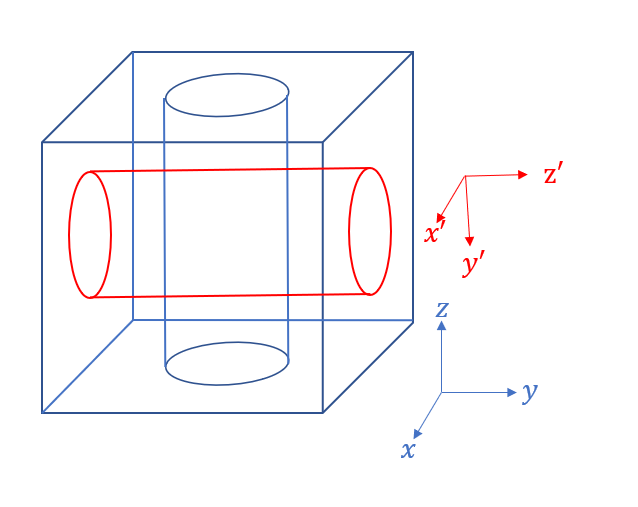
\includegraphics[scale=0.5]{Picture/2}
\end{figure}
为了方便计算,将坐标轴绕x轴旋转90度,可知坐标的变换关系为
\begin{equation}
	x \to x' \qquad  y \to z' \qquad z\to -y'   
	\qquad
	k_x \to k_x^{'} \qquad k_y\to k_z^{'} \qquad k_z \to -k_y^{'}
\end{equation}
由此可知在新坐标系下
\begin{align}
	H_{TI}^{'}(k')=M(k')\tau_3\sigma_0+Ak_x'\tau_2\sigma_1+Ak_z'\tau_2\sigma_2+Ak_y'\tau_2\sigma_3
\end{align}
其BdG哈密顿量变为
\begin{align}
	\begin{pmatrix}
	H_{TI}'(k')-\mu  & \Delta_e(x'+iy')\\
	\Delta_e(x'-iy')  & \mu-H_{TI}'(k')
\end{pmatrix}
\end{align}
由对易关系可知其角动量$J_{z'}=-i\partial_{\theta}-\frac{1}{2}\sigma_2-\frac{1}{2}s_3$
接下来求解$H_{TI}^{'}(k')$的本征态,为了书写方便,后面统一去掉$'$
\begin{align}
	H_{TI}&=M(k)\tau_3\sigma_0+Ak_x\tau_2\sigma_1+Ak_y\tau_2\sigma_3\\
	&=
	\begin{pmatrix}
		M(k) &0& -iAk_y & -iAk_x &\\
		0 &M(k) & -iAk_x & iAk_y\\
		iAk_y& iAk_x &-M(k) &0 \\
		iAk_x & -iAk_y &0 &-M(k)
	\end{pmatrix}
\end{align}
可以找到其与算符$\tau_3\sigma_2$对易,因此可以在其本征态下块对角,可以得到
\begin{align}
	\begin{pmatrix}
		-M(k) & Ak_{-} &0&0\\
		Ak_+ &M(k) &0&0 \\
		0&0&-M(k)&-Ak_+\\
		0&0&-Ak_-&M(k)
	\end{pmatrix}
\end{align}
由此可以得到其四个本征态为
\begin{align}
	\psi_{1}^+=
	\frac{1}{c}
	\begin{pmatrix}
		-i(E+M(k))\\
		E+M(k)\\
		iAke^{-i\theta}\\
		Ake^{-i\theta}
	\end{pmatrix}\qquad
	\psi_{1}^-=
	\frac{1}{d}
\begin{pmatrix}
	-i(-E+M(k))\\
	-E+M(k)\\
	iAke^{-i\theta}\\
	Ake^{-i\theta}
\end{pmatrix}
\end{align}

\begin{align}
		\psi_{2}^+=
		\frac{1}{c}
	\begin{pmatrix}
		i(E+M(k))\\
		E+M(k)\\
		iAke^{i\theta}\\
		-Ake^{i\theta}
	\end{pmatrix}
\qquad
\psi_{2}^-=
\frac{1}{d}
\begin{pmatrix}
	i(-E+M(k))\\
	-E+M(k)\\
	iAke^{i\theta}\\
	-Ake^{i\theta}
\end{pmatrix}
\end{align}
然后计算Berry connection 
\begin{align}
	A_{\theta}^{1+}=\frac{2A^2k^2}{c^2}
		\qquad   
		A_{\theta}^{2+}=-\frac{2A^2k^2}{c^2}\\
		A_{\theta}^{1-}=\frac{2A^2k^2}{d^2}
		\qquad
		A_{\theta}^{2-}=-\frac{2A^2k^2}{d^2}\\
		A_{\theta}^{1+1-}=\frac{2A^2k^2}{cd}
		\qquad
		A_{\theta}^{2+2-}=-\frac{2A^2k^2}{cd}
\end{align}
然后计算角动量的投影,即
\begin{align}
	S^{\dagger}J_zS=S^{\dagger}[-i\partial_{\theta}-\frac{1}{2}\sigma_2-\frac{1}{2}s_3]S
\end{align}
\begin{align}
	S^{\dagger}[-i\partial_{\theta}]S=-i\partial_{\theta}-s_0
	\begin{pmatrix}
		A_{\theta}^{1+} &&A_{\theta}^{1+1-}&\\
		&A_{\theta}^{2+}&&A_{\theta}^{2+2-}\\
		A_{\theta}^{1-1+}&&A_{\theta}^{1-}&\\
		&A_{\theta}^{2-2+}&&A_{\theta}^{2-}
	\end{pmatrix}
\end{align}
\begin{normalsize}
\begin{align}
	&S^{\dagger}\frac{1}{2}\sigma_2S=\frac{1}{2}s_0
	\begin{pmatrix}
			\bra{\psi_{1}^{+}}\\
			\bra{\psi_{2}^{+}}\\
			\bra{\psi_{1}^{-}}\\
			\bra{\psi_{2}^{-}}
	\end{pmatrix}
\begin{pmatrix}
	&-i&&\\
	i&&&\\
	&&&-i\\
	&&i&
\end{pmatrix}
\begin{pmatrix}
			\ket{\psi_{1}^{+}} &\ket{\psi_{2}^{+}} &
			\ket{\psi_{1}^{-}}&\ket{\psi_{2}^{-}}
\end{pmatrix}\\ \nonumber
&=\frac{1}{2}s_0
\begin{pmatrix}
	\frac{2(E+M(k))^2-2A^2k^2}{c^2} &0 & \frac{-4A^2k^2}{cd} &0	\\
	0&\frac{-2(E+M(k))^2+2A^2k^2}{c^2} &0 &\frac{4A^2k^2}{cd} \\
	\frac{-4A^2k^2}{cd} &0 &\frac{2(-E+M(k))^2-2A^2k^2}{d^2} &0\\
	0&\frac{4A^2k^2}{cd} &0 &\frac{-2(-E+M(k))^2+2A^2k^2}{d^2}
\end{pmatrix}\\
&=\frac{1}{2}s_0
\begin{pmatrix}
	1-2A_{\theta}^{1+}  &0 &-2A_{\theta}^{1+1-}&0\\
	0&-1-2A_{\theta}^{2+}&0&-2A_{\theta}^{2+2-}\\
	-2A_{\theta}^{1-1+} &0 &1-2A_{\theta}^{1-}&0\\
	0&-2A_{\theta}^{2-2+} &0 &-1-2A_{\theta}^{2-}
\end{pmatrix}
\end{align}
\end{normalsize}



\begin{align}
			S^{\dagger}\frac{1}{2}s_3S=\frac{1}{2}s_3
\end{align}
由此可以得到投影之后的角动量为
\begin{align}
				J_z^{proj}=-i\partial_{\theta}-\frac{1}{2}
				\begin{pmatrix}
					1&&&\\
					&-1&&\\
					&&1&\\
					&&&-1
				\end{pmatrix}
			-\frac{1}{2}
			\begin{pmatrix}
				1&&&\\
				&1&&\\
				&&-1&\\
				&&&-1
			\end{pmatrix}
\end{align}
后面求解$H_{BdG}^{proj}$的过程与之前一样,可知在$\{\ket{\psi_{1}^{+}}_e,\ket{\psi_{1}^{+}}_h\}$中角动量为
\begin{align}
	J_z^{re}=-i\partial_{\theta}-\frac{1}{2}-\frac{1}{2}\begin{pmatrix}
		1&\\
		&-1
	\end{pmatrix}
\end{align}
最终可以得到
\begin{align}
	E_j=\frac{\Delta_e}{k_F}(j+\frac{1}{2}-A_{\theta}^{1+})
\end{align}
因为$A_{\theta}^{1+}$的值为正,所以可以得到其零能解出现在角动量j=0的位置。
\section*{Conclusion}
通过完整计算$J_z$投影之后的结果,找到了之前角动量不为整数的问题。但是这里的计算似乎表明不管系数是否变号,其角动量的相变点都在$J_z=0$处。之前讨论中提到可能与角动量的定义有关,这一点我还没有想明白。
\par 
对于各向异性的情况,即考虑$k_x,k_y$前面的系数不相等的时候,其费米面不再是一个圆,而是类似于椭圆。其拓扑相变点同样发生在其Berry phase为$\pi$的地方。对于$H_{TI}=M(k)\tau_3\sigma_0+A_1k_x\tau_2\sigma_1+A_2k_y\tau_2\sigma_2$,其中一个能量本征态为
\begin{align}
	\psi_1=
	\frac{1}{a}
	\begin{pmatrix}
		E+m(k)
		\\0\\0\\
		iA_1k_x-A_2k_y
	\end{pmatrix}
\end{align}
可求得
\begin{align}
	A_{k_x}=\frac{A_1A_2k_y}{a^2}\qquad
	A_{k_y}=-\frac{A_1A_2k_x}{a^2}
\end{align}
其在费米面处的方程为$E^2=M(k)^2+A_1^2k_x^2+A_2^2k_y^2$
\begin{align}
	\int_{FS}A_{k_x}dk_x+A_{k_y}dk_y=\iint(\frac{\partial A_{k_y}}{\partial k_x}-\frac{\partial A_{k_x}}{\partial k_y})dk_xdk_y
\end{align}
用Mathematical计算了一下
\begin{figure}[H]
	\centering
	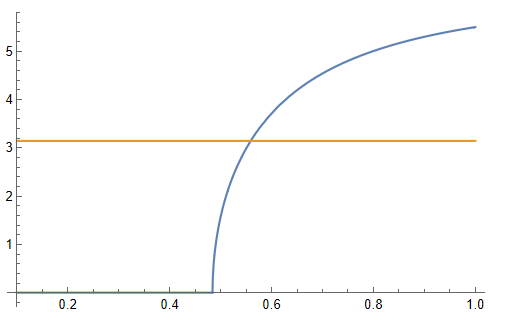
\includegraphics[scale=0.5]{Picture/3}
\end{figure}
A1=A2
\begin{figure}[H]
	\centering
	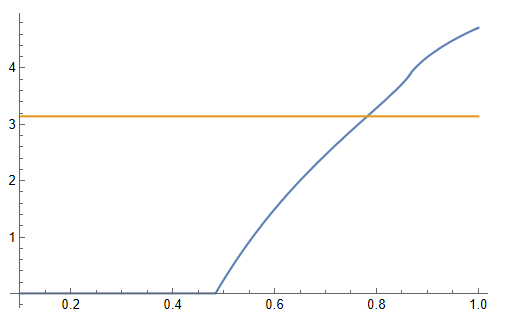
\includegraphics[scale=0.5]{Picture/4}
\end{figure}
A1:A2=2:1
\begin{figure}[H]
	\centering
	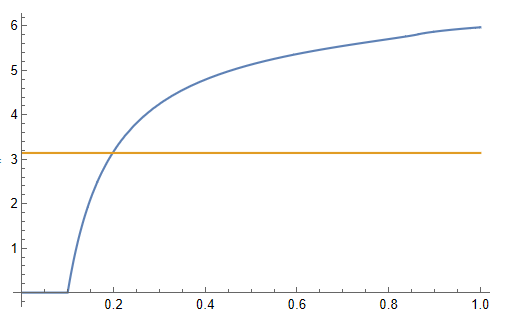
\includegraphics[scale=0.5]{Picture/5}
\end{figure}
A1:A2=10:1
\par 
似乎随着A1:A2差别的增大,拓扑相变点的能量先增大又减少。


\end{document}